\documentclass[reqno, twoside, a4paper,10pt]{amsart}
\usepackage{amsmath}
\usepackage{amssymb}
\usepackage{tikz}
\usetikzlibrary{patterns,decorations.pathreplacing,calligraphy}
\usetikzlibrary{decorations.pathmorphing}
\tikzset{bullet/.style={
shape = circle,fill = black, inner sep = 0pt, outer sep = 0pt, minimum size = 0.4em, line width = 0pt, draw=black!100}}
\tikzset{rectangle/.style={
shape = rectangle,fill = white, inner sep = 0pt, outer sep = 0pt, minimum size = 0.4em, line width = 0.1em, draw=black!100}}
\tikzset{smallbullet/.style={
shape = circle,fill = black, inner sep = 0pt, outer sep = 0pt, minimum size = 0.15em, line width = 0pt, draw=black!100}}
\tikzset{circle/.style={
shape = circle,fill = none, inner sep = 0pt, outer sep = 0pt, minimum size = 0.4em, line width = 0.5pt, draw=black!100}}
\tikzset{empty/.style={
shape = circle,fill = white, inner sep = 0pt, outer sep = 0pt, minimum size = 0.35em, line width = 0pt, draw=white!100}}
\tikzset{xmark/.style={
shape = x,fill = white, inner sep = 0pt, outer sep = 0pt, minimum size = 0em, line width = 0pt, draw=white!100}}
\tikzset{longrectangle/.style={
inner sep = 1em,
% The shape:
rectangle,
% The size:
minimum size=1em,
% The border:
very thick,
draw=black!100, % 50% red and 50% black,
% and that mixed with 50% white
% The filling:
%top color=white, % a shading that is white at the top...
%bottom color=red!50!black!20, % and something else at the bottom
% Font
}}
\tikzset{label distance=-0.15em}
\tikzset{every label/.append style = {font = \scriptsize}}
\tikzset{labelAbove/.style={label={[xshift=-.5\mylength]above:#1}}}
\tikzset{labelBelow/.style={label={[xshift=-.5\mylength]below:#1}}}
\usepackage{tikz-cd}
\tikzcdset{every label/.append style = {font = \normalsize}}

\begin{document}

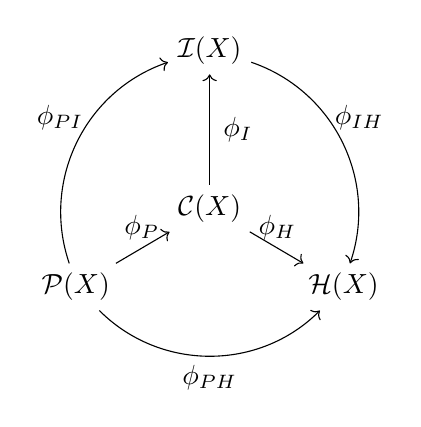
\begin{tikzpicture}[scale=2]
\node[] (C) at (0,0) [] {$\mathcal{C}(X)$};
\node[] (I) at (0,1) [] {$\mathcal{I}(X)$};
\node[] (P) at (-0.85,-0.5) [] {$\mathcal{P}(X)$};
\node[] (H) at (0.85,-0.5) [] {$\mathcal{H}(X)$};

\node[] (phi_I) at (-0.01,0.5) [label=right:{\normalsize $\phi_I$}] {};
\node[] (phi_P) at (-0.43,-0.3) [label=above:{\normalsize $\phi_P$}] {};
\node[] (phi_H) at (0.43,-0.3) [label=above:{\normalsize $\phi_H$}] {};

\node[] (phi_PI) at (-0.95,0.4) [label=above:{\normalsize $\phi_{PI}$}] {};
\node[] (phi_IH) at (0.95,0.4) [label=above:{\normalsize $\phi_{IH}$}] {};
\node[] (phi_PH) at (0,-0.9) [label=below:{\normalsize $\phi_{PH}$}] {};

\draw[->] (P)--(C);
\draw[->] (C)--(I);
\draw[->] (C)--(H);

\draw[->] (P) to [bend left=45] (I);
\draw[->] (I) to [bend left=45] (H);
\draw[->] (P) to [bend right=45] (H);
\end{tikzpicture}

\end{document}